\documentclass[12pt, a4paper]{article}

\usepackage[utf8]{inputenc}
\usepackage[T1]{fontenc}
\usepackage[french]{babel}
\usepackage{geometry}
\usepackage{hyperref}
\usepackage{booktabs}
\usepackage{array}
\usepackage{tabularx}
\usepackage{enumitem}
\usepackage{fancyhdr}
\usepackage{parskip}
\usepackage{listings}
\usepackage{lmodern}
\usepackage{graphicx}
\usepackage{caption}
\usepackage{float}
\usepackage{titlesec}
\usepackage{microtype}

\geometry{margin=2.5cm}

\hypersetup{
  colorlinks=true,
  linkcolor=black,
  urlcolor=black
}

\pagestyle{fancy}
\fancyhf{}
\rhead{\textit{Logbook — Estimateur de plaques malaisiennes}}
\lhead{\textit{Machine Learning Project}}
\rfoot{\thepage}

\lstset{
  basicstyle=\ttfamily\small,
  backgroundcolor=\color{gray!8},
  frame=single,
  rulecolor=\color{gray!40},
  breaklines=true,
  columns=fullflexible,
}

\usepackage{xcolor}

\title{
  \vspace{-1cm}
  {\Large \textbf{Logbook — Projet Machine Learning}} \\[0.5cm]
  {\large Estimation du prix des plaques d'immatriculation spéciales en Malaisie} \\[0.3cm]
  {\normalsize \textit{Journal de bord — mis à jour à chaque étape du projet}}
}
\author{}
\date{\today}

% ══════════════════════════════════════════════════════════════════════════════
\begin{document}
\maketitle
\tableofcontents
\newpage

% ══════════════════════════════════════════════════════════════════════════════
\section{Contexte et objectif du projet}

\subsection{Le marché des plaques spéciales en Malaisie}

En Malaisie, les plaques d'immatriculation ne sont pas simplement des identifiants administratifs. Il existe un marché secondaire très actif où certaines plaques se vendent à des prix considérables, parfois plusieurs millions de ringgits malaisiens (RM). Ce phénomène est profondément ancré dans la culture locale, notamment sous l'influence de la communauté chinoise malaisienne qui accorde une grande importance à la numérologie.

Les critères qui rendent une plaque précieuse sont multiples : la rareté du numéro (un seul chiffre est bien plus rare que quatre), les patterns visuels (palindromes, chiffres répétés), et surtout la symbolique culturelle des chiffres. Le 8 est le chiffre le plus valorisé car il sonne comme ``prospérité'' en cantonais. Le 4, à l'inverse, sonne comme ``mort'' et est généralement évité. Ces plaques sont vendues aux enchères ou à prix fixe sur des plateformes spécialisées.

\subsection{Objectif du projet}

L'objectif est de construire un modèle de machine learning capable d'estimer le prix d'une plaque d'immatriculation malaisienne à partir de son texte brut uniquement. Le cas d'usage concret est simple : on croise une plaque dans la rue, on la note ou on la photographie, et on veut savoir combien elle vaut approximativement sur le marché.

Ce projet est un problème de \textbf{régression supervisée} : à partir de features extraites du texte de la plaque, on prédit une valeur numérique continue (le prix en RM).

% ══════════════════════════════════════════════════════════════════════════════
\section{Étape 1 — Exploration initiale de la base de données}

\subsection{Description de la source}

La base de données initiale est un fichier CSV (\texttt{licence\_plate\_price.csv}) contenant deux colonnes :
\begin{itemize}
  \item \texttt{plate} : le texte brut de la plaque (ex: \texttt{WMA 4}, \texttt{EV 8888}, \texttt{QS 6 W})
  \item \texttt{price} : le prix au format texte tel qu'affiché sur le site source (ex: \texttt{RM 3,800})
\end{itemize}

Les données ont été collectées par web scraping depuis le site \textbf{Motor Trader} (\url{https://www.motortrader.com.my}), une plateforme malaisienne spécialisée dans la vente de véhicules et de plaques d'immatriculation spéciales. Le fichier contient \textbf{3\,420 entrées} à l'état brut.

\subsection{Analyse exploratoire (EDA)}

Un script d'exploration complet a été développé (\texttt{explore\_data.py}) pour analyser la qualité des données avant tout nettoyage. Ce script génère un rapport visuel multi-panneaux incluant une heatmap des valeurs manquantes, la distribution des prix, et une répartition par tranches de prix.

\begin{table}[H]
\centering
\begin{tabular}{lr}
\toprule
\textbf{Métrique} & \textbf{Valeur} \\
\midrule
Entrées totales & 3\,420 \\
Valeurs NaN (colonne \texttt{plate}) & 0 \\
Valeurs NaN (colonne \texttt{price}) & 0 \\
Prix invalides (format POA) & 107 \\
Plaques mal formées & 5 \\
Prix minimum (entrées valides) & RM 500 \\
Prix maximum (entrées valides) & RM 1\,880\,000 \\
Prix médian & RM 5\,800 \\
Prix moyen & RM 25\,806 \\
\bottomrule
\end{tabular}
\caption{Statistiques initiales de la base de données}
\end{table}

La figure~\ref{fig:quality} présente la répartition des entrées valides et invalides, ainsi que le détail des suppressions effectuées lors du nettoyage.

\begin{figure}[H]
  \centering
  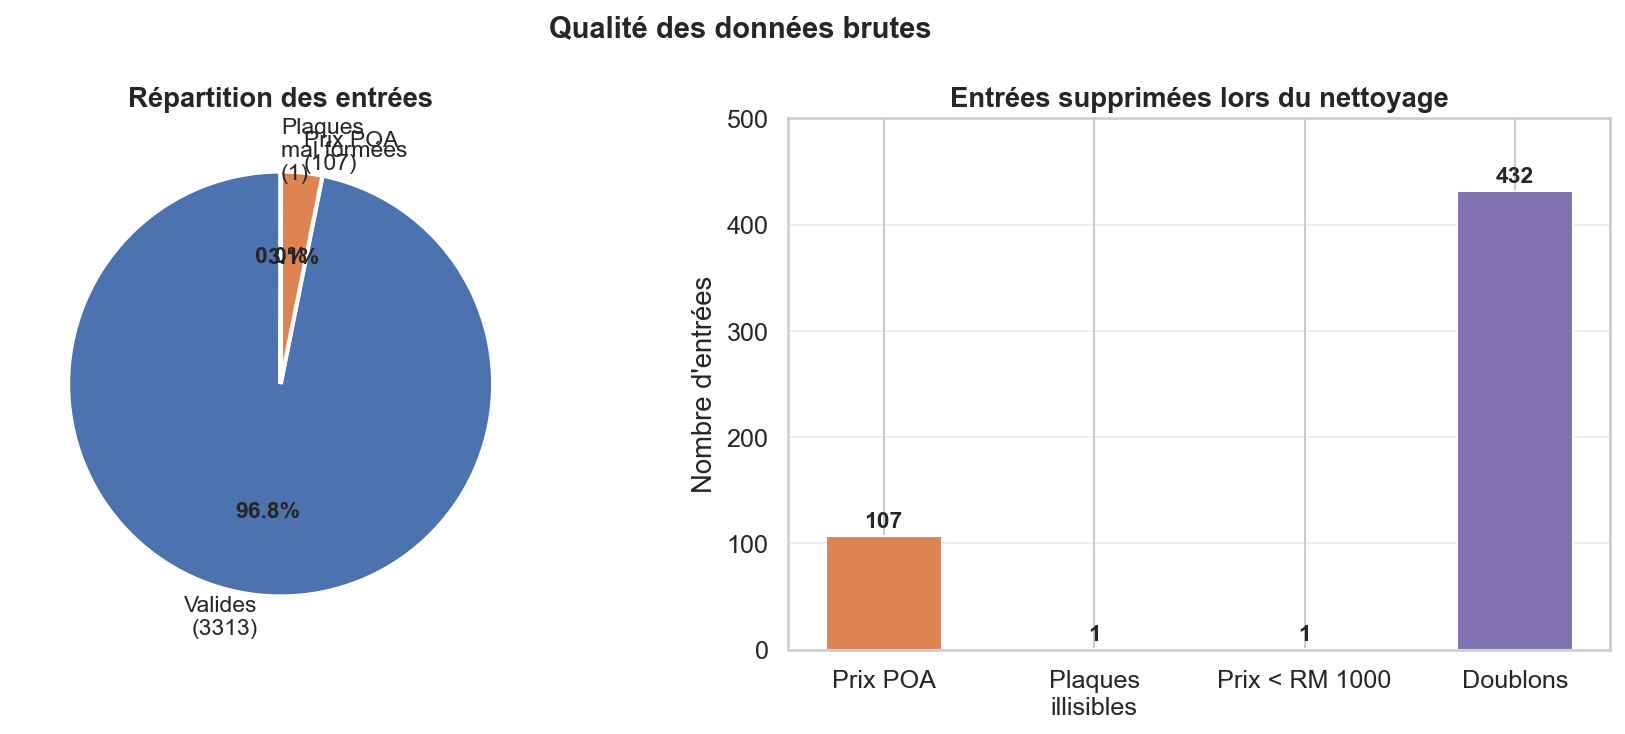
\includegraphics[width=\textwidth]{fig1_data_quality.png}
  \caption{Qualité des données brutes : répartition valides/invalides et détail des suppressions}
  \label{fig:quality}
\end{figure}

La figure~\ref{fig:distrib} montre la distribution des prix en échelle logarithmique. Cette représentation est la plus informative car elle révèle la structure réelle de la distribution, masquée en échelle linéaire par les quelques plaques à prix extrêmes.

\begin{figure}[H]
  \centering
  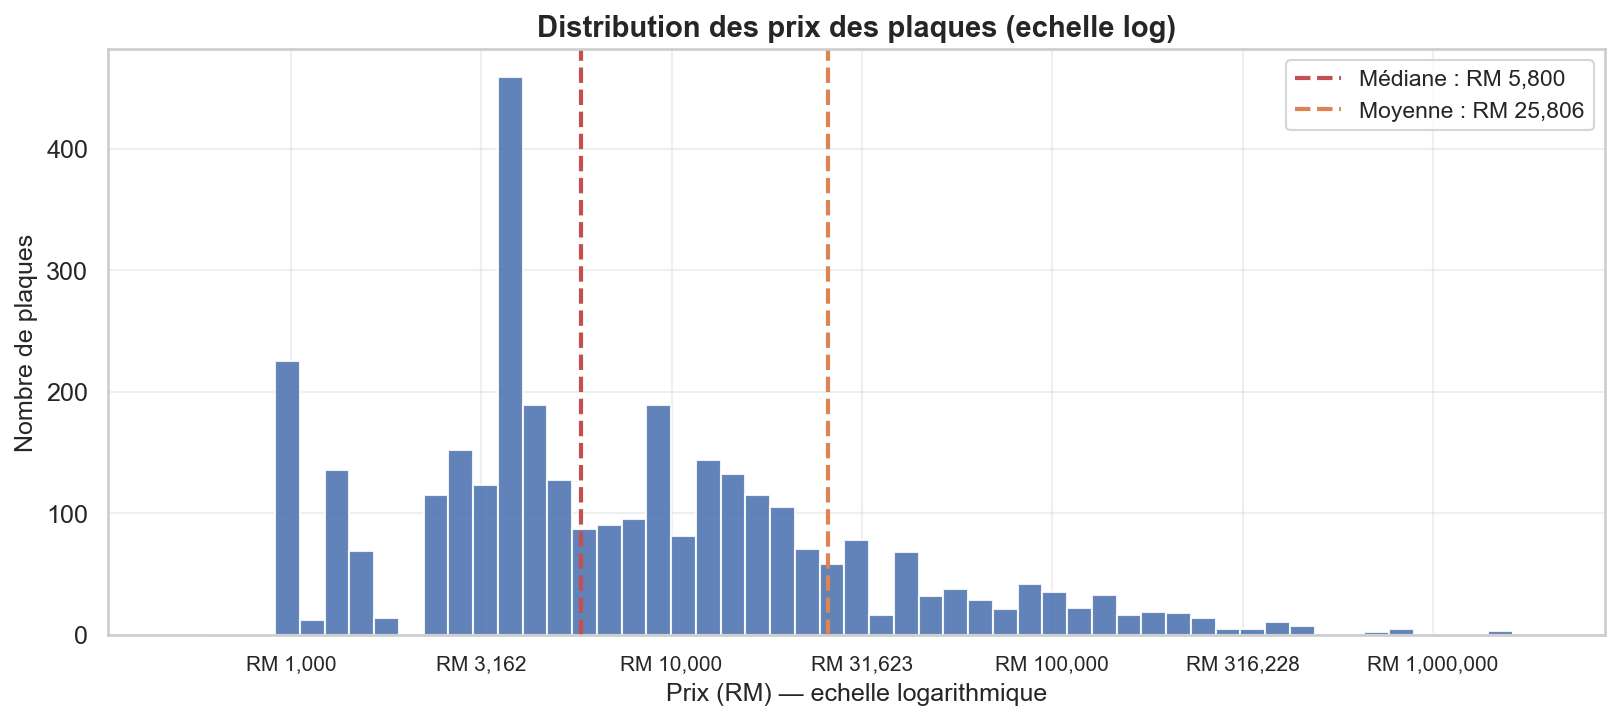
\includegraphics[width=\textwidth]{fig2_price_distribution.png}
  \caption{Distribution des prix en échelle logarithmique — médiane et moyenne}
  \label{fig:distrib}
\end{figure}

La figure~\ref{fig:brackets} détaille la répartition des plaques par tranche de prix, ce qui permet de visualiser concrètement la concentration du marché.

\begin{figure}[H]
  \centering
  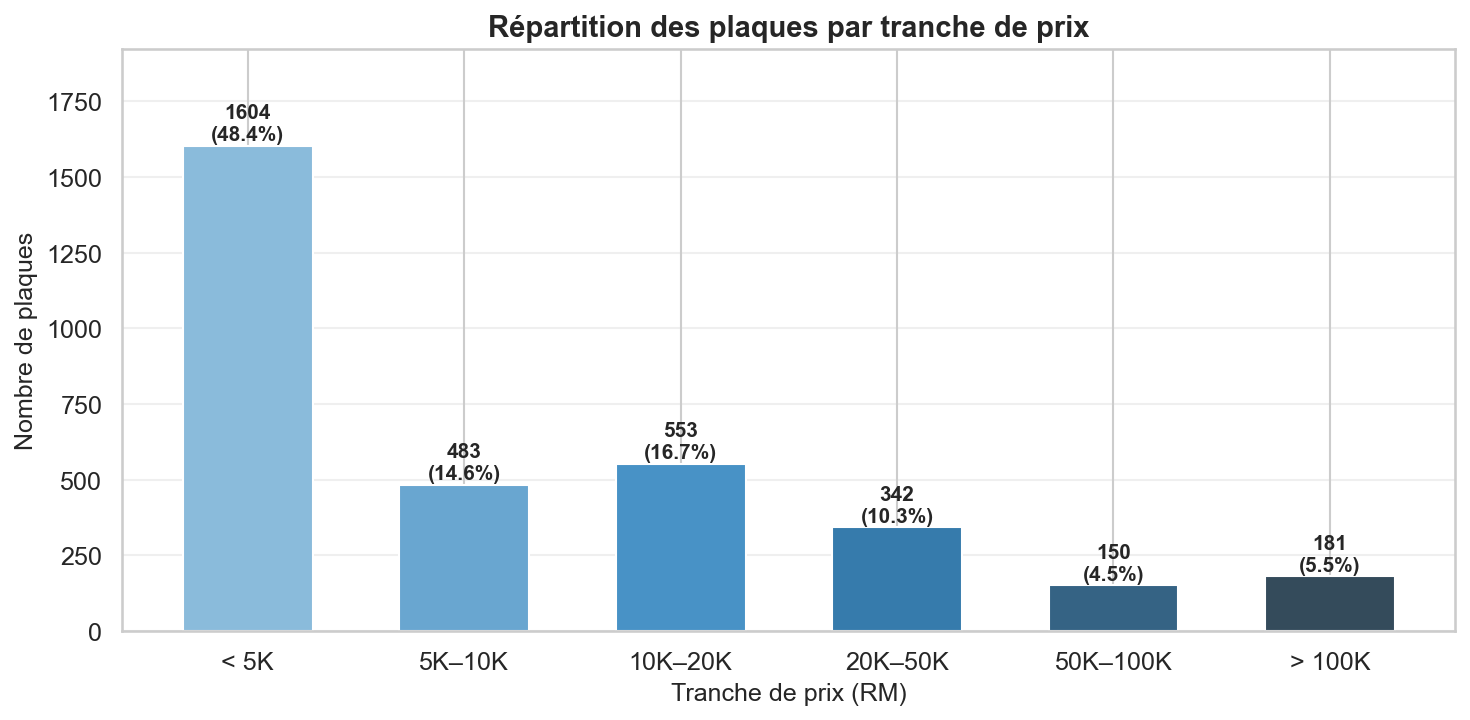
\includegraphics[width=0.85\textwidth]{fig3_price_brackets.png}
  \caption{Répartition des plaques par tranche de prix (RM)}
  \label{fig:brackets}
\end{figure}

\subsection{Observations clés}

\textbf{Distribution des prix très asymétrique.} La médiane (RM 5\,800) est très éloignée de la moyenne (RM 25\,806). Cela signifie que la grande majorité des plaques se vendent entre RM 2\,000 et RM 10\,000, mais quelques plaques extrêmement rares tirent la moyenne vers le haut. Cette asymétrie est visible sur l'histogramme : la distribution est fortement étalée vers la droite (\textit{right-skewed}). En échelle logarithmique, la distribution devient beaucoup plus symétrique, ce qui suggère qu'une transformation log du prix pourrait améliorer les performances du modèle.

\textbf{Absence de NaN.} Aucune valeur manquante au sens strict (NaN) n'a été détectée. Les problèmes de qualité sont d'une autre nature : des prix non numériques (POA) et des plaques avec des caractères invalides.

\textbf{Prix POA (Price On Application).} 107 plaques ont un prix affiché comme ``POA'', c'est-à-dire ``prix sur demande''. Ces plaques ne peuvent pas être utilisées pour l'entraînement car elles n'ont pas de valeur numérique. Il est probable que ces plaques soient parmi les plus rares et les plus chères du marché, ce qui introduit un biais dans notre dataset (voir section~\ref{sec:critique}).

% ══════════════════════════════════════════════════════════════════════════════
\section{Étape 2 — Nettoyage des données}

\subsection{Stratégie de nettoyage}

Le nettoyage a été réalisé dans \texttt{clean\_data.py}. La philosophie adoptée est de \textbf{supprimer plutôt que d'imputer} : avec seulement deux colonnes (plaque et prix), il n'y a pas de valeur à imputer — une entrée sans prix valide ou avec une plaque illisible est simplement inutilisable.

\subsection{Opérations effectuées}

\paragraph{1. Suppression des prix POA.}
Les 107 entrées avec \texttt{price = "POA"} ont été supprimées. Ces entrées représentent 3,1\% du dataset. Elles ne peuvent pas contribuer à l'entraînement d'un modèle de régression.

\paragraph{2. Nettoyage des plaques mal formées.}
Cinq plaques présentaient des problèmes de format :
\begin{itemize}
  \item Caractères spéciaux illisibles : \texttt{VP? 9} — supprimée (1 cas)
  \item Alias entre parenthèses : \texttt{JAB 4 (VIP 3)}, \texttt{CCG4 (CCC4)}, etc. — nettoyées par regex pour ne garder que la plaque principale (4 cas)
  \item Minuscules : \texttt{bqb 666} — converties en majuscules
\end{itemize}

\paragraph{3. Normalisation des espaces.}
Deux plaques présentaient des espaces multiples (\texttt{VKU~~8228}, \texttt{VMJ~~8228}). Ces espaces ont été normalisés à un espace simple.

\paragraph{4. Suppression du prix anormalement bas.}
Une seule entrée avait un prix inférieur à RM 1\,000 : \texttt{JYV1103} à RM 500. Ce prix est anormalement bas par rapport au reste du marché (le minimum habituel est autour de RM 1\,000--2\,000). Cette entrée a été supprimée comme probable erreur de saisie.

\paragraph{5. Suppression des doublons.}
432 doublons ont été détectés et supprimés (conservation de la première occurrence). Ce nombre élevé — 12,6\% du dataset — est significatif et mérite une explication détaillée (voir ci-dessous).

\subsection{Le problème des doublons}

432 doublons représentent une proportion importante du dataset. Après analyse, il apparaît que la source de données liste plusieurs fois les mêmes plaques, probablement parce que les données ont été collectées à plusieurs reprises depuis le même site sans déduplication entre les collectes. Les doublons sont des entrées strictement identiques (même plaque, même prix), ce qui confirme qu'il s'agit d'un artefact de collecte et non de vraies plaques différentes avec le même numéro.

Ce point est important pour interpréter la taille réelle du dataset : les 3\,420 entrées initiales ne représentent en réalité que 2\,879 plaques uniques.

\subsection{Résultat final}

\begin{table}[H]
\centering
\begin{tabular}{lr}
\toprule
\textbf{Opération} & \textbf{Entrées supprimées} \\
\midrule
Prix POA & 107 \\
Plaques illisibles & 1 \\
Prix $<$ RM 1\,000 & 1 \\
Doublons & 432 \\
\midrule
\textbf{Total supprimé} & \textbf{541} \\
\textbf{Entrées finales} & \textbf{2\,879} \\
\bottomrule
\end{tabular}
\caption{Bilan du nettoyage}
\end{table}

Le fichier nettoyé \texttt{licence\_plate\_price\_cleaned.csv} contient deux colonnes : \texttt{plate} (texte normalisé en majuscules) et \texttt{price} (float en RM).

\subsection{Traitement des outliers de prix}

Une analyse IQR ($\times 3$) identifie 280 entrées au-dessus de RM 57\,300 comme outliers statistiques. Ces entrées n'ont \textbf{pas été supprimées}. En effet, dans ce contexte, un prix de RM 1\,880\,000 pour la plaque \texttt{KH1} n'est pas une erreur — c'est une plaque single digit avec un préfixe très court, légitimement l'une des plus rares du marché. Supprimer ces entrées priverait le modèle d'apprendre les cas extrêmes qui sont précisément les plus intéressants à prédire.

% ══════════════════════════════════════════════════════════════════════════════
\section{Étape 3 — Split train / test}

Le dataset nettoyé a été divisé en deux ensembles distincts avant toute modélisation, conformément aux bonnes pratiques de machine learning. Cette séparation est essentielle pour évaluer les performances du modèle sur des données qu'il n'a jamais vues pendant l'entraînement.

\begin{table}[H]
\centering
\begin{tabular}{lrr}
\toprule
\textbf{Ensemble} & \textbf{Entrées} & \textbf{Proportion} \\
\midrule
Train & 2\,303 & 80\% \\
Test & 576 & 20\% \\
\midrule
Total & 2\,879 & 100\% \\
\bottomrule
\end{tabular}
\caption{Répartition train/test}
\end{table}

Le split a été effectué avec \texttt{shuffle=True} et \texttt{random\_state=42} pour garantir la reproductibilité. Aucune stratification n'a été appliquée (la stratification est utile pour les problèmes de classification avec des classes déséquilibrées, mais moins pertinente pour la régression).

% ══════════════════════════════════════════════════════════════════════════════
\section{Étape 4 — Feature Engineering}

\subsection{Pourquoi le feature engineering est l'étape centrale}

Le modèle ne peut pas travailler directement sur le texte brut \texttt{"EV 8888"}. Il faut transformer cette chaîne de caractères en un vecteur de nombres qui capturent les caractéristiques pertinentes pour le prix. C'est l'étape de \textit{feature engineering}, et dans ce projet elle est particulièrement importante car \textbf{toute l'information disponible est contenue dans le texte de la plaque}.

Contrairement à d'autres projets ML où les features sont déjà présentes dans le dataset (âge, revenu, etc.), ici nous devons les construire entièrement à partir de zéro en nous appuyant sur notre compréhension du marché malaisien.

Toutes les features sont implémentées dans \texttt{features.py}, un module réutilisable importé par \texttt{train.py} et \texttt{predict.py}.

\subsection{Features de structure}

Ces features décrivent la forme brute de la plaque.

\begin{itemize}
  \item \texttt{prefix\_len} : longueur du préfixe lettres. Une plaque comme \texttt{EV 8888} a un préfixe de 2 lettres, \texttt{VPA 6363} en a 3. Les séries à préfixe court sont plus anciennes et donc plus rares. C'est l'une des features les plus discriminantes.
  \item \texttt{num\_digits} : nombre de chiffres dans la plaque. C'est probablement la feature la plus importante : les plaques à 1 chiffre (\texttt{KH1}, \texttt{VR1}) atteignent des prix de plusieurs centaines de milliers à plusieurs millions de RM, tandis que les plaques à 4 chiffres se vendent généralement entre RM 2\,000 et RM 10\,000.
  \item \texttt{total\_len} : longueur totale de la plaque sans espaces.
  \item \texttt{digits\_value} : valeur numérique brute du numéro (ex: \texttt{4} pour \texttt{WMA 4}).
\end{itemize}

\subsection{Features de numérologie et culture malaisienne}

Ces features capturent les croyances culturelles qui influencent directement le marché.

\begin{itemize}
  \item \texttt{lucky\_count} et \texttt{lucky\_ratio} : nombre et proportion de chiffres chanceux (8, 9, 6, 1). Le 8 est le plus valorisé (``prospérité'' en cantonais), suivi du 9 (``longévité''), du 6 (``fluidité'') et du 1 (``premier'', ``unique'').
  \item \texttt{unlucky\_count} : nombre de 4. Le 4 sonne comme ``mort'' (``sì'') en cantonais et mandarin. En théorie, sa présence devrait faire baisser le prix. En pratique, l'analyse montre que ce n'est pas toujours le cas (voir section~\ref{sec:nuances}).
  \item \texttt{digit\_sum} : somme des chiffres, utilisée en numérologie.
  \item \texttt{ends\_8}, \texttt{starts\_8} : indicateurs booléens pour la position du 8.
  \item \texttt{contains\_888}, \texttt{contains\_8888} : la séquence 888 est particulièrement valorisée. \texttt{DFB 888} se vend RM 138\,000, \texttt{JT 888} RM 118\,800.
\end{itemize}

\subsection{Features de patterns visuels}

Ces features capturent l'esthétique et la mémorabilité de la plaque.

\begin{itemize}
  \item \texttt{all\_same} : tous les chiffres sont identiques (ex: 8888, 1111, 9999). Ces plaques sont très recherchées. \texttt{Y 9999} se vend RM 218\,800.
  \item \texttt{is\_palindrome} : le numéro se lit pareil dans les deux sens (ex: 1221, 8558, 9999). \texttt{UU 88} à RM 588\,000 est à la fois palindrome et all\_same.
  \item \texttt{is\_abab} : pattern de répétition ABAB (ex: 1212, 8989, 1313). \texttt{IM 1313} se vend RM 68\,000.
  \item \texttt{max\_repeat} : longueur de la plus longue séquence de chiffres identiques consécutifs. Permet de capturer des cas comme \texttt{888} dans \texttt{SJR 9888} (max\_repeat=3).
\end{itemize}

\subsection{Features de rareté}

\begin{itemize}
  \item \texttt{is\_single} : numéro à 1 chiffre (1--9). Les plaques les plus rares et les plus chères du marché.
  \item \texttt{is\_double} : numéro à 2 chiffres (10--99).
  \item \texttt{is\_round} : multiple de 100 (ex: 100, 400, 1000). Ces numéros ``ronds'' ont une certaine valeur esthétique.
  \item \texttt{is\_short\_prefix} : préfixe de 1 ou 2 lettres, indicateur de série ancienne.
\end{itemize}

\subsection{Validation des features sur la base réelle}

Chaque feature a été vérifiée en cherchant des exemples réels dans la base et en comparant avec les prix observés. Le tableau suivant présente quelques exemples représentatifs :

\begin{table}[H]
\centering
\begin{tabular}{llrp{6cm}}
\toprule
\textbf{Plaque} & \textbf{Prix réel} & \textbf{Features actives} \\
\midrule
\texttt{KH1} & RM 1\,880\,000 & is\_single, prefix\_len=2, all\_same \\
\texttt{T10} & RM 988\,000 & is\_double, prefix\_len=1 \\
\texttt{UU 88} & RM 588\,000 & is\_double, all\_same, is\_palindrome, ends\_8 \\
\texttt{DFB 888} & RM 138\,000 & contains\_888, max\_repeat=3, lucky\_count=3 \\
\texttt{Y 9999} & RM 218\,800 & all\_same, is\_palindrome, lucky\_count=4, prefix\_len=1 \\
\texttt{IM 1313} & RM 68\,000 & is\_abab, lucky\_count=2 \\
\texttt{PSD 999} & RM 21\,300 & all\_same, is\_palindrome, lucky\_count=3, num\_digits=3 \\
\texttt{VPA 6363} & RM 3\,800 & is\_abab, lucky\_count=2, prefix\_len=3 \\
\texttt{VKY 2797} & RM 1\,000 & aucun pattern, unlucky\_count=0, prefix\_len=3 \\
\bottomrule
\end{tabular}
\caption{Exemples de validation des features sur la base réelle}
\end{table}

La cohérence est bonne : les features discriminent bien les plaques rares des communes.

\subsection{Features retirées et justification}
\label{sec:features_retirees}

\paragraph{is\_sequential et is\_rev\_seq.}
Ces deux features détectaient les suites croissantes (ex: 1234, 5678) et décroissantes (ex: 9876, 4321). Elles ont été retirées pour une raison statistique simple : la base ne contient que \textbf{8 cas séquentiels} et \textbf{4 cas décroissants}, soit moins de 0,5\% du dataset. Avec si peu d'exemples, le modèle ne peut pas apprendre un signal fiable — ces features introduiraient du bruit plutôt que de l'information.

De plus, l'analyse montre que le prix d'une plaque séquentielle dépend surtout d'autres features déjà présentes : \texttt{R 8765} vaut RM 26\,800 principalement à cause de son préfixe à 1 lettre (\texttt{prefix\_len=1}), pas parce que c'est une suite décroissante. La feature \texttt{is\_rev\_seq} n'apporterait donc pas d'information supplémentaire dans ce cas.

\textit{À améliorer :} avec une base de données plus large incluant davantage de plaques séquentielles, ces features pourraient être réintégrées.

\subsection{Nuances importantes}
\label{sec:nuances}

\paragraph{Le chiffre 4 ne pénalise pas toujours.}
La feature \texttt{unlucky\_count} repose sur l'hypothèse que le 4 fait baisser le prix. L'analyse sur la base réelle montre que ce n'est pas systématique : \texttt{DT 4} se vend RM 259\,800 et \texttt{A 44 A} RM 218\,800 malgré la présence de 4. Quand la plaque est courte et rare, le marché valorise la rareté avant la numérologie. La feature est conservée mais le modèle devra apprendre cette interaction avec d'autres features (notamment \texttt{num\_digits} et \texttt{prefix\_len}).

\paragraph{Redondance partielle de all\_same.}
Pour les plaques à 1 chiffre (\texttt{is\_single=1}), la feature \texttt{all\_same} est mécaniquement vraie et donc redondante. Elle apporte de l'information uniquement pour les plaques à 3--4 chiffres (ex: 999, 8888). Un modèle comme Gradient Boosting gère bien cette redondance partielle.

% ══════════════════════════════════════════════════════════════════════════════
\section{Critique de la base de données}
\label{sec:critique}

\subsection{Limites identifiées}

\paragraph{1. Taille modeste.}
2\,879 entrées après nettoyage est une taille limitée pour un problème de régression avec une variable cible couvrant un ratio de 1 à 1\,880 (de RM 1\,000 à RM 1\,880\,000). Les cas extrêmes — plaques très chères et très communes — sont sous-représentés, ce qui rend difficile l'apprentissage des frontières de prix.

\paragraph{2. Doublons à la source.}
432 doublons (12,6\% du dataset initial) indiquent une collecte non rigoureuse. La base provient probablement d'un scraping répété du même site sans déduplication entre les collectes. Cela signifie que le dataset réel est encore plus petit qu'il n'y paraît.

\paragraph{3. Sous-représentation de certains patterns.}
Les plaques séquentielles (8 cas) et décroissantes (4 cas) sont trop rares pour être apprises correctement. D'autres patterns culturels spécifiques pourraient également être sous-représentés. Une base plus large permettrait d'inclure ces features.

\paragraph{4. Absence de contexte temporel.}
Les prix des plaques évoluent avec le marché (enchères, tendances économiques, popularité de certains chiffres). La base ne contient aucune date, il est donc impossible de savoir si les prix sont récents ou anciens, ni de modéliser l'évolution temporelle des prix.

\paragraph{5. Biais lié aux prix POA.}
107 plaques ont un prix ``sur demande'' (POA) et ont dû être exclues. Ces plaques sont probablement parmi les plus rares et les plus chères du marché — leur exclusion crée un biais vers le bas dans les estimations pour les plaques très rares. Le modèle risque de sous-estimer les prix des plaques les plus exceptionnelles.

\paragraph{6. Absence d'information contextuelle.}
Le prix d'une plaque peut dépendre de facteurs non capturés dans notre dataset : l'état de la plaque (neuve vs. déjà immatriculée), la région d'émission, la popularité du préfixe dans une communauté particulière, ou encore la date de l'enchère. Ces informations ne sont pas disponibles.

% ══════════════════════════════════════════════════════════════════════════════
% ══════════════════════════════════════════════════════════════════════════════
\section{Étape 5 — Choix du modèle}
\label{sec:choix_modele}

\subsection{Caractéristiques du problème}

Avant de choisir un modèle, il faut caractériser précisément le problème pour identifier les contraintes auxquelles le modèle devra répondre :

\begin{itemize}
  \item \textbf{Type de problème :} régression supervisée — on prédit une valeur numérique continue (le prix en RM).
  \item \textbf{Taille du dataset :} 2\,303 exemples d'entraînement. C'est un dataset de taille modeste.
  \item \textbf{Nature des features :} mixte — features booléennes (0/1), entières (nombre de chiffres, longueur du préfixe), et continues (ratio de chiffres chanceux, valeur numérique). Aucune feature catégorielle ordinale complexe.
  \item \textbf{Distribution de la cible :} très asymétrique (right-skewed). La majorité des prix se concentre entre RM 2\,000 et RM 10\,000, mais quelques plaques atteignent plusieurs centaines de milliers voire des millions de RM. Cette asymétrie est un défi pour les modèles qui minimisent l'erreur quadratique moyenne (MSE), car ils seront fortement influencés par les valeurs extrêmes.
  \item \textbf{Interactions non-linéaires :} les features interagissent de façon complexe. Par exemple, la présence du chiffre 4 (\texttt{unlucky\_count}) ne pénalise le prix que si la plaque n'est pas par ailleurs très rare (\texttt{num\_digits} élevé, \texttt{prefix\_len} long). Ces interactions ne peuvent pas être capturées par un modèle linéaire.
\end{itemize}

\subsection{Analyse des candidats}

\paragraph{Régression linéaire.}
Inadaptée. Les relations entre les features et le prix ne sont pas linéaires — un single digit ne vaut pas simplement ``prefix\_len $\times$ coefficient''. La régression linéaire ne peut pas capturer les interactions entre features ni les effets multiplicatifs. Éliminée d'emblée.

\paragraph{Support Vector Regression (SVR).}
Peu adapté. Sensible à l'échelle des features, nécessite une normalisation soigneuse, et ne gère pas bien les interactions complexes sur des données tabulaires avec de nombreuses features binaires. Les performances sur ce type de problème sont généralement inférieures aux méthodes ensemblistes.

\paragraph{Réseau de neurones (MLP).}
Surdimensionné pour ce problème. Avec seulement 2\,303 exemples d'entraînement et 20 features, un réseau de neurones risque fortement le surapprentissage. De plus, les réseaux de neurones ne sont pas les plus efficaces sur des données tabulaires de petite taille — les méthodes ensemblistes les surpassent généralement dans ce contexte.

\paragraph{Random Forest Regressor.}
Bon candidat. Robuste aux outliers, gère naturellement les interactions entre features, ne nécessite pas de normalisation, et est peu sensible aux hyperparamètres. Cependant, le Random Forest a une limitation importante pour ce problème : il prédit en faisant la \textbf{moyenne des prédictions de ses arbres}, ce qui le pousse à régresser vers la moyenne et à sous-estimer les valeurs extrêmes. Or, les plaques les plus chères sont précisément les plus intéressantes à prédire correctement.

\paragraph{Gradient Boosting Regressor (GBR).}
Meilleur choix pour ce problème. Contrairement au Random Forest qui construit ses arbres en parallèle de façon indépendante, le Gradient Boosting construit les arbres \textbf{séquentiellement}, chaque arbre corrigeant les erreurs du précédent. Cette approche lui permet de mieux capturer les cas difficiles, notamment les valeurs extrêmes. Il gère très bien les features avec peu de valeurs uniques (booléennes) et les interactions non-linéaires complexes.

\subsection{Décision et justification}

\textbf{Modèle principal : Gradient Boosting Regressor.}
\textbf{Modèle de référence (baseline) : Random Forest Regressor.}

Le Random Forest servira de baseline pour évaluer le gain apporté par le Gradient Boosting. Si les deux modèles donnent des performances similaires, cela indiquera que le problème est bien capturé par les features et que le choix du modèle est secondaire.

\subsection{Transformation de la variable cible}

La distribution des prix étant fortement asymétrique, le modèle sera entraîné sur \textbf{log(prix)} plutôt que sur le prix brut. Cette transformation présente deux avantages :

\begin{enumerate}
  \item Elle rend la distribution de la cible plus symétrique, ce qui facilite l'apprentissage et réduit l'influence disproportionnée des valeurs extrêmes sur la fonction de perte.
  \item Elle est cohérente avec la perception humaine des prix : une erreur de RM 5\,000 sur une plaque à RM 10\,000 est bien plus grave qu'une erreur de RM 5\,000 sur une plaque à RM 500\,000. En travaillant en log, on minimise l'erreur relative plutôt que l'erreur absolue.
\end{enumerate}

Les prédictions seront reconverties en RM (via $e^{\hat{y}}$) pour l'évaluation finale et l'interface utilisateur.

% ══════════════════════════════════════════════════════════════════════════════
% ══════════════════════════════════════════════════════════════════════════════
\section{Étape 6 — Entraînement et évaluation des modèles}
\label{sec:training}

\subsection{Pipeline d'entraînement}

L'entraînement est réalisé dans \texttt{train.py}. Le pipeline complet est le suivant :

\begin{enumerate}
  \item Chargement de \texttt{train.csv} et \texttt{test.csv}
  \item Extraction des features via \texttt{features.py} (\texttt{build\_feature\_matrix})
  \item Encodage du préfixe lettres par \texttt{LabelEncoder}
  \item Transformation de la cible : $y = \log(\text{prix})$
  \item Entraînement des deux modèles
  \item Évaluation sur le jeu de test (reconversion $\hat{y} \rightarrow e^{\hat{y}}$ pour les métriques en RM)
  \item Sauvegarde du meilleur modèle dans \texttt{models/best\_model.pkl}
\end{enumerate}

\subsection{Résultats}

\begin{table}[H]
\centering
\begin{tabular}{lrrr}
\toprule
\textbf{Modèle} & \textbf{MAE (RM)} & \textbf{R² (log)} & \textbf{MAPE} \\
\midrule
Gradient Boosting & 8\,259 & 0.9180 & 31.1\% \\
\textbf{Random Forest} & \textbf{5\,906} & \textbf{0.9206} & \textbf{28.7\%} \\
\bottomrule
\end{tabular}
\caption{Comparaison des performances sur le jeu de test}
\end{table}

\subsection{Analyse des résultats}

\paragraph{Le Random Forest surpasse le Gradient Boosting.}
Ce résultat est contre-intuitif par rapport à notre analyse préalable. Plusieurs explications sont possibles :

\begin{itemize}
  \item \textbf{Taille du dataset :} avec seulement 2\,303 exemples d'entraînement, le Gradient Boosting — qui est un algorithme plus complexe avec plus d'hyperparamètres — est plus difficile à optimiser et peut souffrir d'un léger surapprentissage. Le Random Forest, plus robuste par construction (bagging), se comporte mieux sur les petits datasets.
  \item \textbf{Structure des features :} la majorité des features sont binaires (0/1). Le Random Forest gère très efficacement ce type de features car chaque arbre peut créer des partitions nettes sur ces valeurs. Le Gradient Boosting, qui construit des arbres peu profonds (\texttt{max\_depth=4}), peut avoir du mal à capturer toutes les interactions.
\end{itemize}

\paragraph{Interprétation des métriques.}
\begin{itemize}
  \item \textbf{R² = 0.92 :} le modèle explique 92\% de la variance des prix (en échelle log). C'est un très bon résultat pour un problème avec une distribution aussi étalée.
  \item \textbf{MAE = RM 5\,906 :} en moyenne, le modèle se trompe de RM 5\,906. Rapporté à la médiane du marché (RM 5\,800), cela représente une erreur d'environ 100\% sur les plaques bon marché, mais une erreur bien plus faible en proportion sur les plaques chères.
  \item \textbf{MAPE = 28.7\% :} l'erreur relative moyenne est de 28,7\%. C'est acceptable pour un marché aussi hétérogène, mais indique que le modèle a du mal sur certaines tranches de prix.
\end{itemize}

\paragraph{Modèle retenu.}
Le \textbf{Random Forest} est retenu comme modèle final et sauvegardé dans \texttt{models/best\_model.pkl}.

\subsection{Visualisations}

La figure~\ref{fig:predvsreal} compare les prix prédits aux prix réels pour les deux modèles. Les points proches de la diagonale rouge indiquent de bonnes prédictions.

\begin{figure}[H]
  \centering
  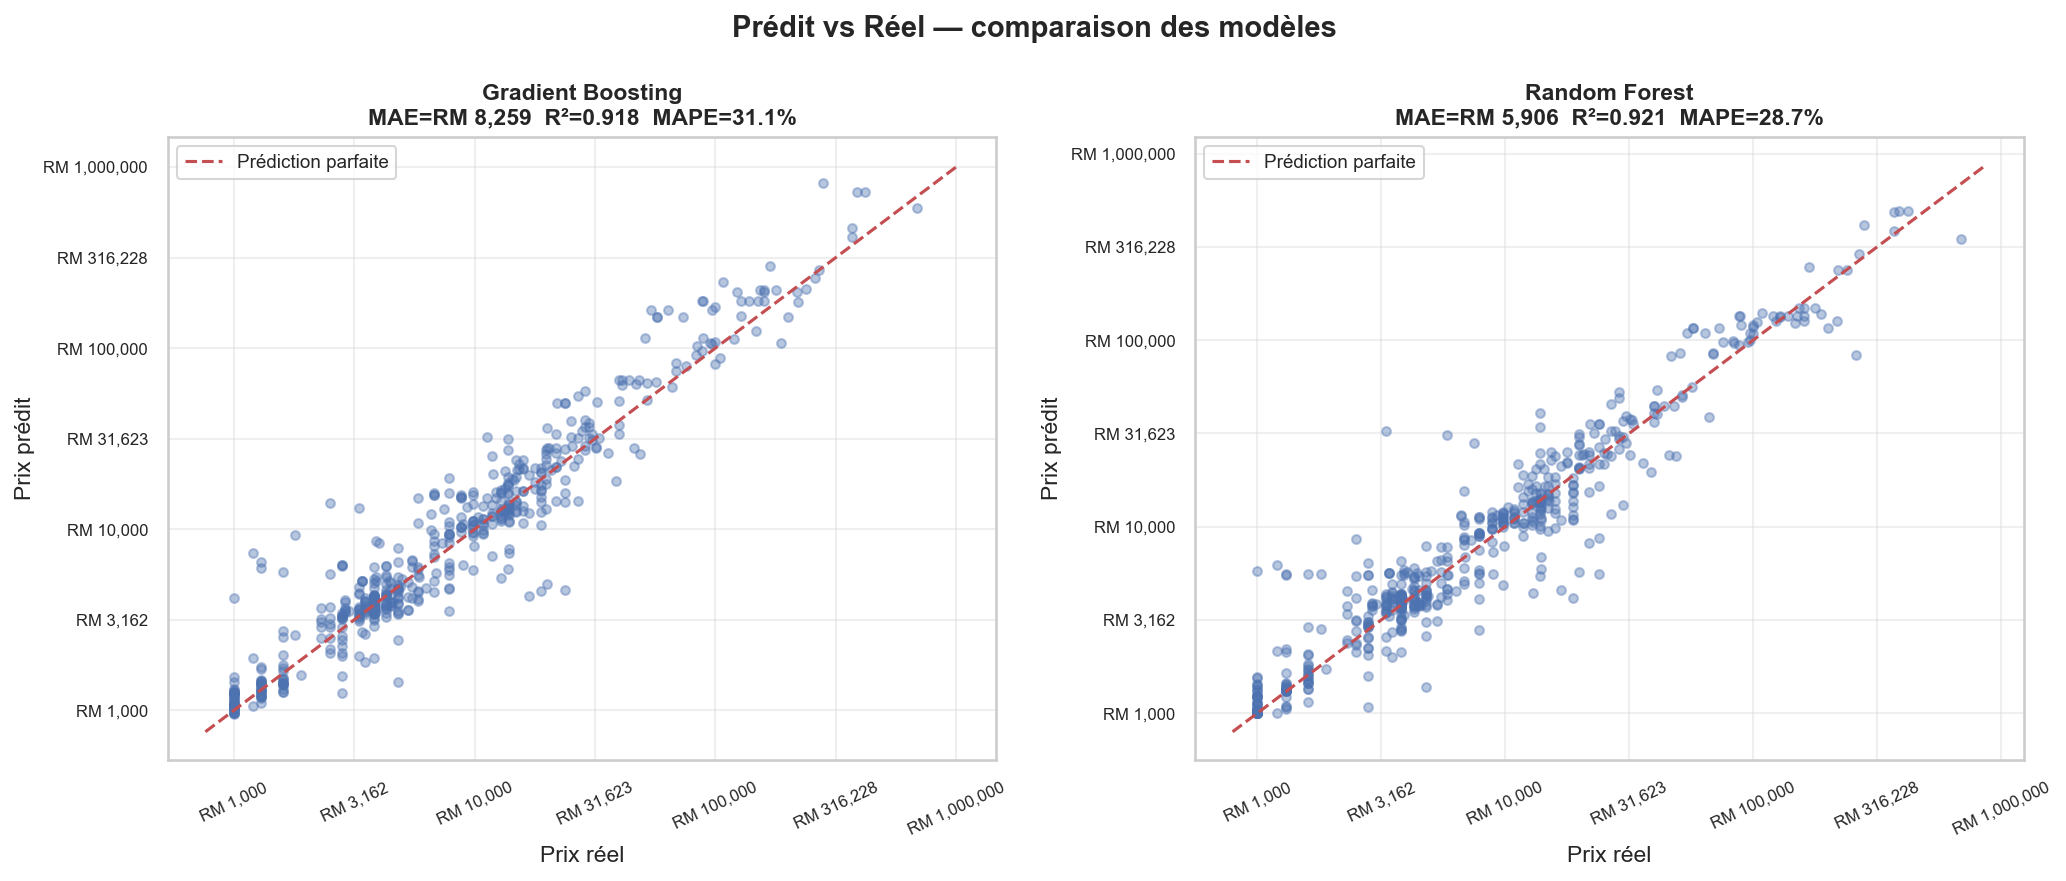
\includegraphics[width=\textwidth]{fig4_pred_vs_real.png}
  \caption{Prix prédit vs prix réel — Gradient Boosting et Random Forest (échelle log)}
  \label{fig:predvsreal}
\end{figure}

La figure~\ref{fig:importance} présente les features les plus importantes selon le Random Forest.

\begin{figure}[H]
  \centering
  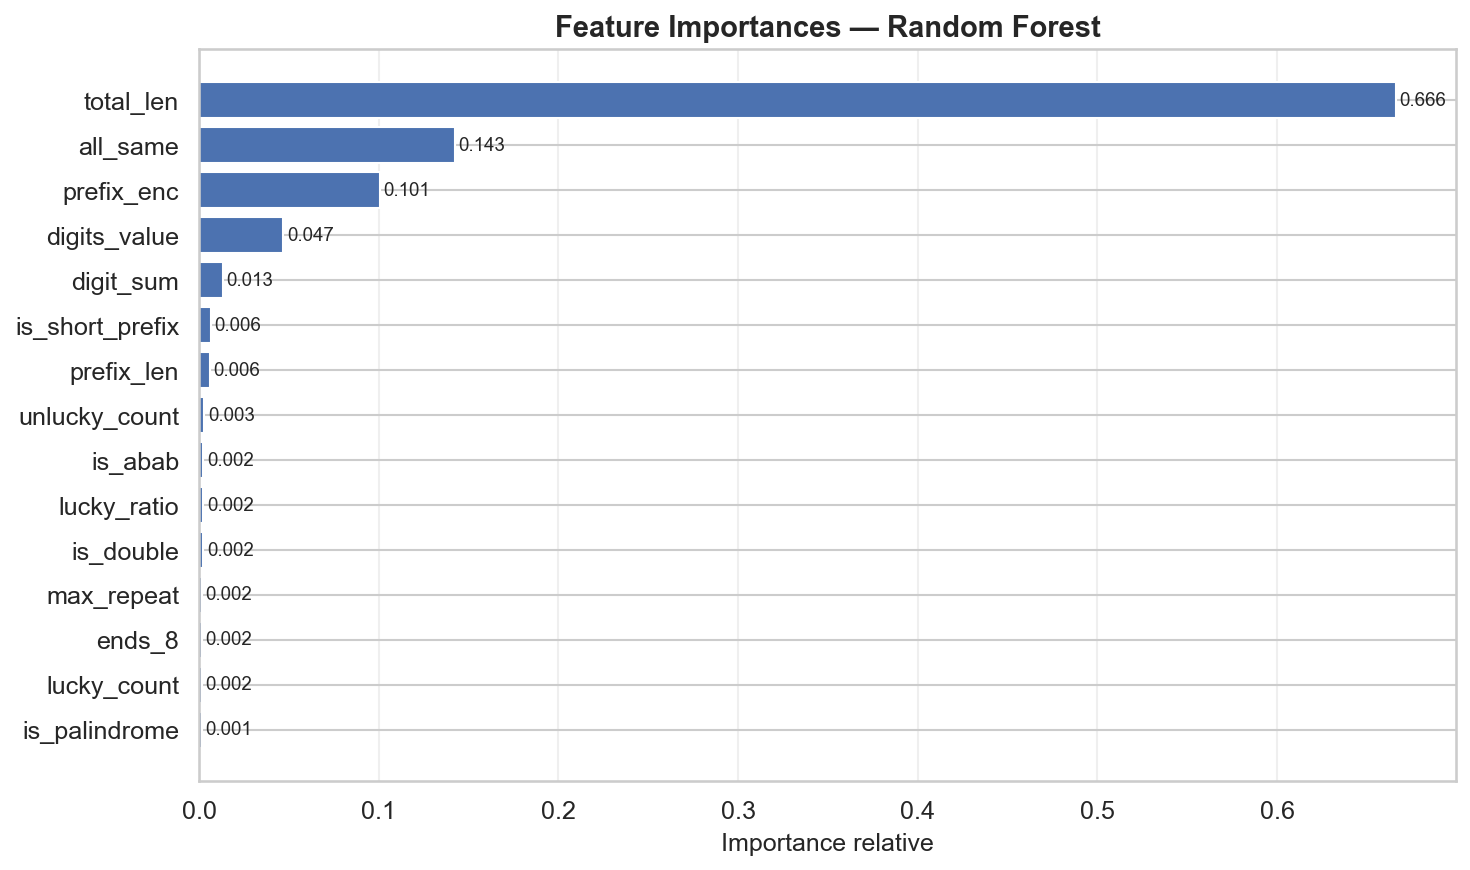
\includegraphics[width=0.9\textwidth]{fig5_feature_importance.png}
  \caption{Feature importances — Random Forest}
  \label{fig:importance}
\end{figure}

% ══════════════════════════════════════════════════════════════════════════════
\section{Étape 7 — Amélioration du modèle (V2)}
\label{sec:v2}

\subsection{Motivations}

Après les résultats de la V1 (Random Forest, MAE=RM 5\,906, R²=0.9206), trois pistes d'amélioration ont été explorées simultanément :

\begin{enumerate}
  \item \textbf{Features d'interaction manuelle} : aider le modèle en créant explicitement les combinaisons de features les plus importantes.
  \item \textbf{LightGBM} : implémentation optimisée du gradient boosting, plus efficace que le GBR de sklearn.
  \item \textbf{Stacking} : combiner Random Forest et LightGBM avec un méta-modèle Ridge.
\end{enumerate}

\subsection{Nouvelles features d'interaction}

Six features d'interaction ont été ajoutées au vecteur de features existant (21 features de base → 27 features au total) :

\begin{itemize}
  \item \texttt{rarity\_score} : $\frac{1}{\text{num\_digits} \times \text{prefix\_len}}$ — score de rareté combinée. Plus le numéro est court et le préfixe court, plus ce score est élevé.
  \item \texttt{same\_and\_lucky} : \texttt{all\_same} $\times$ \texttt{lucky\_count} — distingue 8888 (très chanceux) de 1111 (all\_same mais peu chanceux).
  \item \texttt{single\_short} : \texttt{is\_single} $\times$ (\texttt{prefix\_len} $\leq$ 2) — capture l'effet exponentiel d'un single digit avec préfixe court.
  \item \texttt{palin\_lucky} : \texttt{is\_palindrome} $\times$ \texttt{lucky\_count} — palindrome avec chiffres chanceux.
  \item \texttt{digits\_x\_repeat} : \texttt{num\_digits} $\times$ \texttt{max\_repeat} — capture les cas comme 8888 (4 chiffres, tous répétés).
  \item \texttt{unlucky\_weighted} : \texttt{unlucky\_count} $\times$ \texttt{num\_digits} — la pénalité du 4 est pondérée par la longueur : sur une plaque longue, le 4 pénalise plus que sur une plaque courte et rare.
\end{itemize}

\subsection{Résultats V2}

\begin{table}[H]
\centering
\begin{tabular}{lrrr}
\toprule
\textbf{Modèle} & \textbf{MAE (RM)} & \textbf{R² (log)} & \textbf{MAPE} \\
\midrule
V1 — Random Forest (référence) & 5\,906 & 0.9206 & 28.7\% \\
\midrule
V2 — Random Forest & 5\,644 & 0.9149 & 30.9\% \\
V2 — LightGBM & 5\,849 & 0.9127 & 32.9\% \\
\textbf{V2 — Stacking (RF + LightGBM)} & \textbf{5\,605} & 0.9158 & 31.7\% \\
\bottomrule
\end{tabular}
\caption{Comparaison V1 vs V2}
\end{table}

\subsection{Analyse}

\paragraph{Le stacking est le meilleur modèle V2 sur la MAE.}
Le stacking (RF + LightGBM avec méta-modèle Ridge) atteint une MAE de RM 5\,605, soit une réduction de RM 301 par rapport à la V1. Les features d'interaction contribuent à cette amélioration en aidant le modèle à mieux capturer les effets combinés.

\paragraph{Trade-off MAE vs R² vs MAPE.}
Un résultat contre-intuitif apparaît : le R² de la V2 est légèrement inférieur à celui de la V1 (0.9158 vs 0.9206), et la MAPE est plus élevée (31.7\% vs 28.7\%). Cela signifie que le stacking réduit les grosses erreurs absolues (MAE) mais est moins précis en proportion sur les plaques bon marché. Ce trade-off est acceptable pour notre cas d'usage : une erreur de RM 300 sur une plaque à RM 1\,000 est plus gênante qu'une erreur de RM 5\,000 sur une plaque à RM 500\,000.

\paragraph{LightGBM décevant.}
LightGBM, pourtant réputé très performant sur les données tabulaires, ne surpasse pas le Random Forest ici. Cela confirme que la taille modeste du dataset (2\,303 exemples) favorise les méthodes ensemblistes simples comme le Random Forest, moins sensibles aux hyperparamètres.

\subsection{Modèle final retenu}

Le \textbf{Stacking (RF + LightGBM)} est retenu comme modèle final V2, sauvegardé dans \texttt{train\_v2/models/best\_model\_v2.pkl}.

\subsection{Visualisations V2}

\begin{figure}[H]
  \centering
  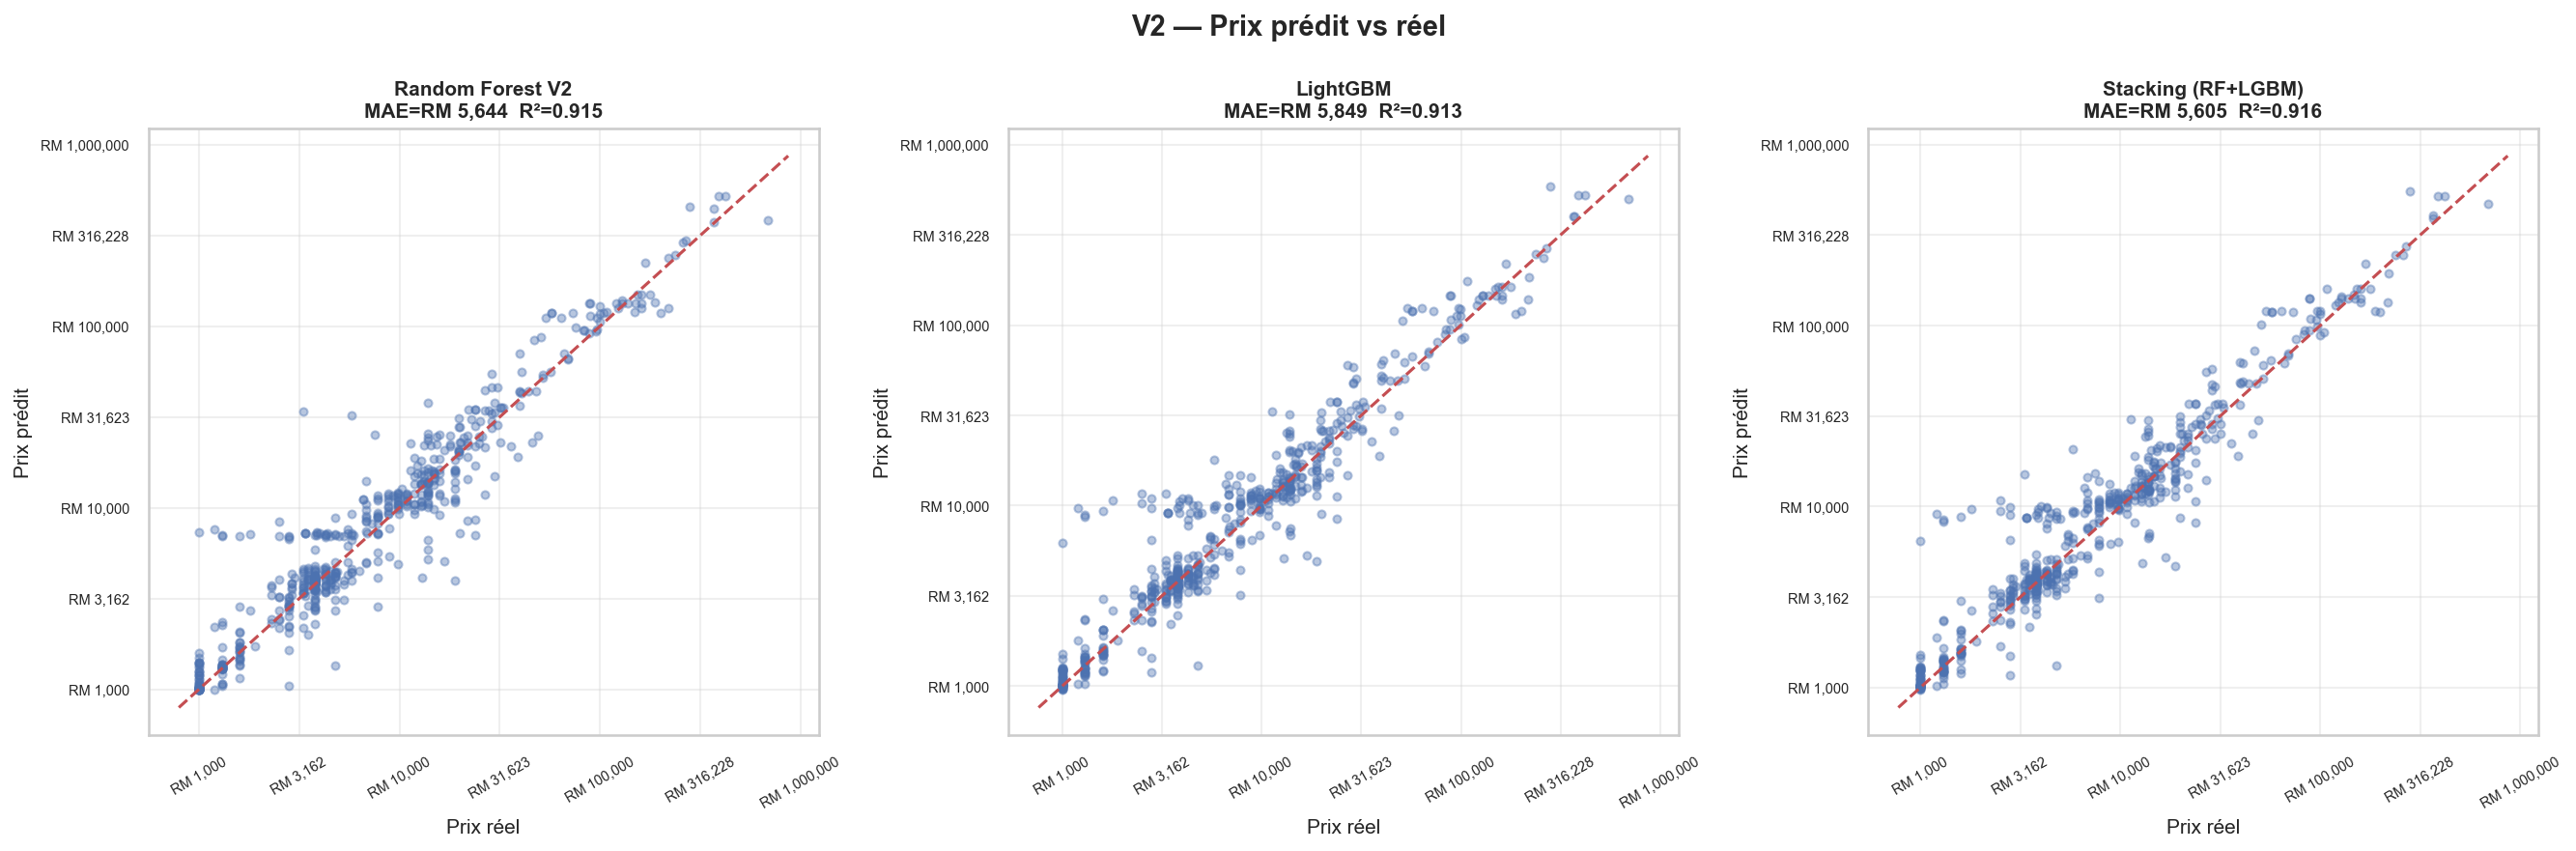
\includegraphics[width=\textwidth]{fig_v2_pred_vs_real.png}
  \caption{V2 — Prix prédit vs réel pour les trois modèles}
  \label{fig:v2pred}
\end{figure}

\begin{figure}[H]
  \centering
  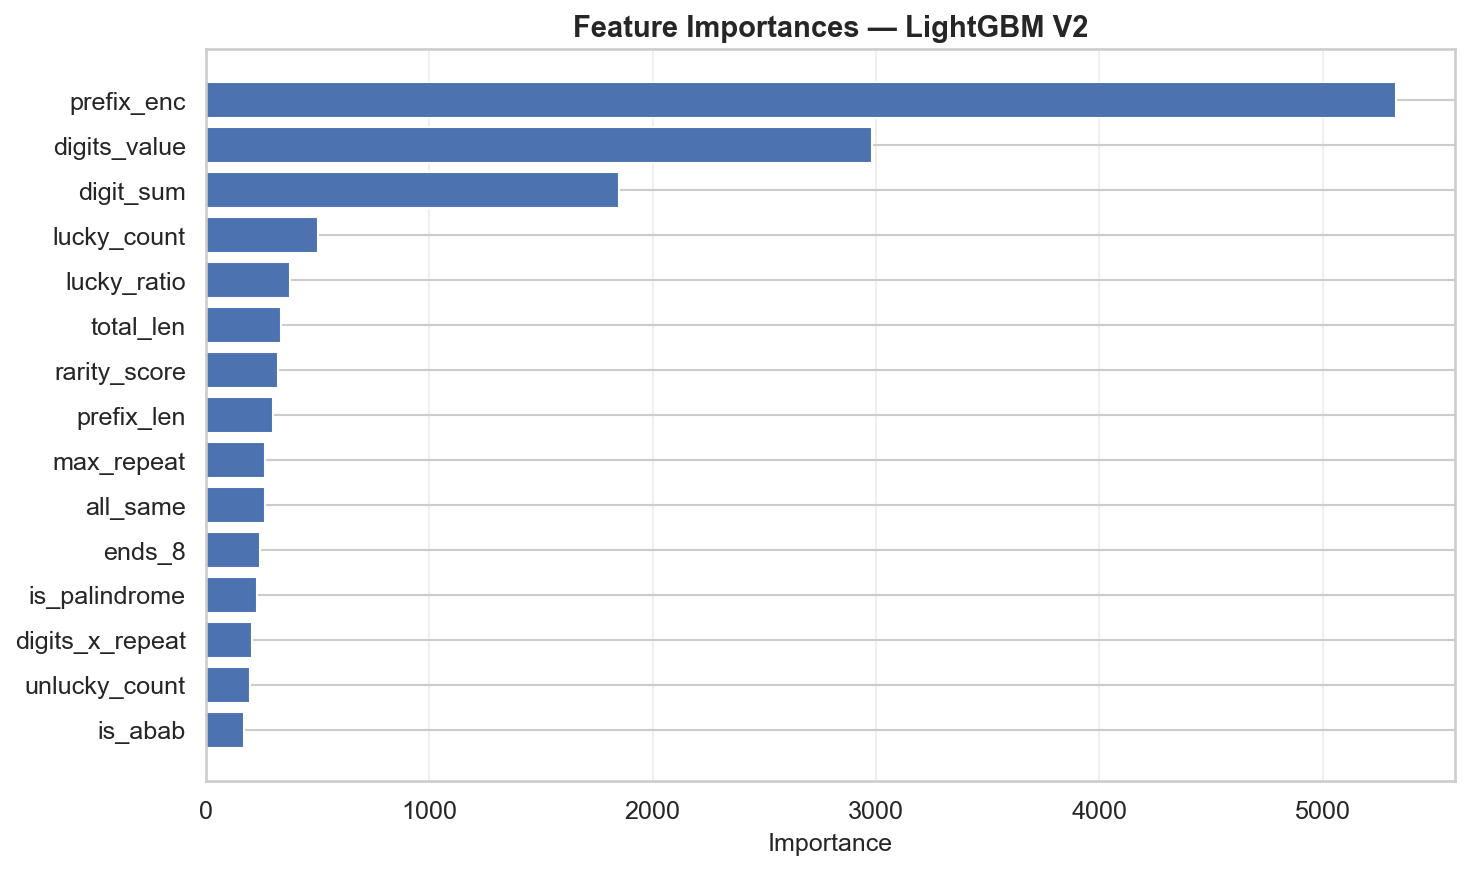
\includegraphics[width=0.9\textwidth]{fig_v2_feature_importance.png}
  \caption{V2 — Feature importances LightGBM (incluant les features d'interaction)}
  \label{fig:v2imp}
\end{figure}

% ══════════════════════════════════════════════════════════════════════════════
\section{Prochaines étapes}

\begin{itemize}[leftmargin=2cm]
  \item[$\boxtimes$] Entraînement des modèles V1 (Gradient Boosting + Random Forest)
  \item[$\boxtimes$] Évaluation sur le jeu de test (MAE, R², MAPE)
  \item[$\boxtimes$] Amélioration V2 (features d'interaction + LightGBM + Stacking)
  \item[$\boxtimes$] Analyse des feature importances
% ══════════════════════════════════════════════════════════════════════════════
\section{Étape 8 — Interface de prédiction}
\label{sec:predict}

\subsection{Description}

Le script \texttt{predict.py} constitue l'interface utilisateur finale du projet. Il charge le modèle V2 (Stacking RF+LightGBM) et permet d'estimer le prix de n'importe quelle plaque en ligne de commande.

\textbf{Deux modes d'utilisation :}
\begin{itemize}
  \item Mode direct : \texttt{python predict.py "WMA 4"}
  \item Mode interactif : \texttt{python predict.py} (saisie en boucle)
\end{itemize}

Pour chaque plaque, le script affiche le prix estimé et une explication des facteurs qui influencent la valeur.

\subsection{Exemples de prédictions}

\begin{table}[H]
\centering
\begin{tabular}{lrrl}
\toprule
\textbf{Plaque} & \textbf{Prix estimé} & \textbf{Prix réel} & \textbf{Facteurs principaux} \\
\midrule
\texttt{KH 1}    & RM 1\,448\,048 & RM 1\,880\,000 & single digit, préfixe court \\
\texttt{EV 8888} & RM 56\,791     & RM 68\,800     & 8888, all\_same, préfixe court \\
\texttt{VPA 6363}& RM 3\,088      & RM 3\,800      & pattern ABAB \\
\texttt{WMA 4}   & RM 52\,770     & —              & single digit, pénalité 4 \\
\bottomrule
\end{tabular}
\caption{Exemples de prédictions du modèle final}
\end{table}

Les estimations sont dans le bon ordre de grandeur. L'écart sur \texttt{KH 1} (RM 432\,000) s'explique par le fait que les plaques les plus extrêmes sont sous-représentées dans le dataset d'entraînement.
  \item[$\square$] Dashboard Streamlit (optionnel)
\end{itemize}

\end{document}
